\documentclass[9pt,twocolumn,twoside]{../../styles/osajnl}
\usepackage{fancyvrb}
\journal{i524}
\title{Google BigQuery - A data warehouse for large-scale data analytics}

\author[1]{Sagar Vora}

\affil[1]{School of Informatics and Computing, Bloomington, IN 47408, U.S.A.}

\dates{\today}

\ociscodes{BigQuery, ETL, BigData, Google, Cloud, Database, SaaS, SQL}

% replace this with your url in github/gitlab
\doi{\url{https://github.com/vorasagar7/sp17-i524/paper2/S17-IR-2041/report.pdf}}


\begin{abstract}

There has been an increase in the volume of relational data generated
today through a large number of sources. The large volume of data
forces us to find solutions which can cope with them. Recently several
hybrid approaches like HadoopDB, Hive, etc have been introduced to
handle this large data. Although these have been successful in
handling large data, but their architecture makes them inefficient to
handle suboptimal execution strategies. Moreover this data is the
information that companies would like to explore and analyse quickly
to identify strategic answers to business. Therefore, in order to
solve the problem of traditional database management systems to
support large volumes of data arises Google's BigQuery platform. This
solution runs in cloud, SQL-like queries against massive quantites of
data, providing real time insights about the data. In this paper, we
will analyze the main features of BigQuery that Google offers to
manage large-scale data. \newline
\end{abstract}

% \setboolean{displaycopyright}{true}

\begin{document}

\maketitle

\section{Introduction}
Nowadays, the amount of data being collected, stored and processed
continues to grow rapidly. Therefore high performance and scalability
have become two essentials requirements for data analytics
systems. Querying massive datasets can be time consuming and expensive
without the right hardware and infrastructure. Google BigQuery solves
this problem by enabling super-fast, SQL-like queries against
append-only tables, using the processing power of Google's
infrastructure. Google BigQuery \cite{www-bigquery}
\cite{bigquery-paper} is a cloud web service very attractive for its
ease of use and functionality. It is ideal for businesses that cannot
invest in infrastructure to process a huge amount of information. This
platform allows to store and retrieve large amounts of information in
near real time with main focus on data analysis.

\section{Cloud Computing}
Cloud computing \cite{www-cloudcomputing}
\cite{benchmark-for-cloud-paper} allows access to computing resources
easily scalable and virtualized via the Internet. The use becomes
simpler because users need not to have knowledge, experience or
management of the infrastructure. There are usually three types of
cloud offerings:\begin{itemize} \item Infrastructure as a service
  (IaaS) which provides basic compute and storage resources including
  servers, networking. \item Platform as a service (PaaS) which
  provides a platform allowing users to develop, run and manage
  applications without the complexity of building and maintaning the
  infrastructure typically associated with developing and launching
  apps. \item Software as a Service (SaaS) which refers to one of the
  most known cloud services, which consists of applications running
  directly in the cloud provider. \end{itemize}

\noindent

\section{Google BigQuery}
To solve the problems faced by Hadoop \cite{www-apache-hadoop}
MapReduce \cite{mapreduce-article}, Google developed Dremel
application in order to process large volumes of data. Dremel was
designed to deliver high performance on data which was distributed
across multiple servers and SQL support. But in 2012 at Google I/O
event, it was announced the end of the Dremel and the beginning of
BigQuery which became then the high-performance cloud offering of
google.

\begin{figure}[htbp]
\centering
\fbox{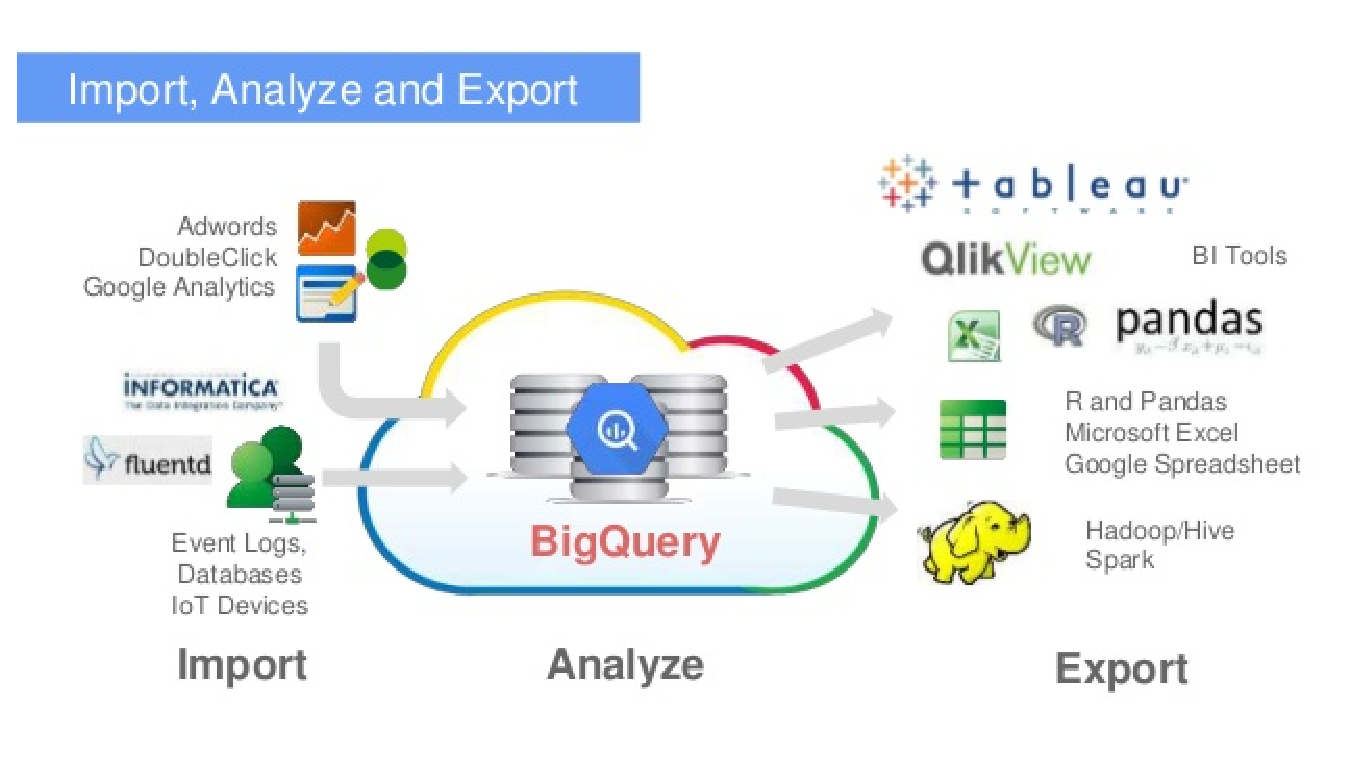
\includegraphics[width=\linewidth]{images/architecture}}
\caption{\cite{www-bigquery-slideshare} System Architecture of BigQuery}
\label{fig:architecture}
\end{figure}

Figure \ref{fig:architecture} shows the system architecture of BigQuery.

\noindent
Google BigQuery \cite{bigquery-paper} platform is a SaaS as a model in
the cloud. It is not a reporting system and does not have an interface
that allows the operation of the information but it is ideal to export
results by Tableau, QlikView, Excel, among others including the tools
of Business Intelligence (BI) as seen in Figure
\ref{fig:architecture}. Projects are top-level containers that store
information about billing and authorized users, and they contain
BigQuery data. When we create a new project, it is identified by a
name, authorized users and data \cite{www-bigquery-documentation}.

Data which is generated from a variety of sources like event logs,
relational databases, IoT devices like sensors, social media websites,
etc is given as an input to BigQuery which processes it to generate
some meaningful anaylsis according to the requirement. The final data
could be represented and exported using Tableau, Qlikview and other BI
tools. It can also be exported on Hadoop system for pararell
processing \ref{fig:architecture}.

\section{Features of BigQuery}
Google BigQuery \cite{www-bigquery} presents some characteristics like Velocity,
Scalability, Security and multiple access methods.

\subsection{Velocity}

BigQuery can process millions of information which is not indexed in seconds
due to columnar storage, and tree architecture as explained below.

\subsection{Columnar Storage}
The data instead of being stored in terms of rows, the data is stored
as columnsand thus storage will be oriented. This will result in
scanning of only the required values, largely reducing latency. This
storage also allows for a higher compression ratio. Google reports
\cite{www-rowvscolumnstorage} that they can achieve columnar
compression ratios of 1:10 as opposed to 1:3 when storing data in a
traditional row based format. The reason behind this is the similarity
of data stored in the columns as the variation is significantly lower
than when the data is stored in rows.

\begin{figure}[htbp]
\centering
\fbox{\includegraphics[width=\linewidth]{images/rowvscolumnstorage}}
\caption{\cite{www-rowvscolumnstorage} Row vs Column Storage}
\label{fig:rowvscolumnarstorage}
\end{figure}

Figure \ref{fig:rowvscolumnarstorage} shows the rows and column
oriented storage.

\subsection{Tree Architecture}
This is used for processing queries and aggregating results across
different nodes. BigQuery is spread across thousands of servers. The
data is sharded across multiple machines
\ref{fig:rowvscolumnarstorage}. This helps retrieve data much
faster. Let us see this with the help of 2 examples.

Here, A is our root server, with B being an intermediate server and C,
D, E being leaf servers having local disk storage.

Example 1: Speed
Statement: List out all the customer names starting with ‘G’

Let us assume Node C contains customer names.  Hence, it is as simple
as traversing A -> B -> C and looking at the datasets Cr1 and Cr2 for
names starting with G. One need not look at A -> B -> D and A ->
E. Hence, in this simple scenario, we have already achieved a search
time of 0.33x that of a typical RDBMS (assuming equal column sizes).

Example 2: Parallel Processing
Statement: Count all the customer names
starting with ‘G’

\begin{itemize}
\item Root A passes the query to intermediate B. \item B translates
  the query to Sum (Count all the customer names starting with
  ‘G’). \item Intermediate B passes this query to Leaf C. \item Leaf C
  has tablets (Horizontal sharded tables) r1 and r2. \item C accesses
  these tablets in parallel, runs quick counts and passes the count of
  Cr1 and Cr2 to B. \item B sums Cr1 and Cr2 and passes it to the root
  A for output. \end{itemize}

Now, if this architecture was scaled to thousands of leaf servers and
hundreds of intermediate servers. This achieves enormous amounts of
parallel processing by utilizing a small percentage of the CPU
processing and Disk I/O of each server as opposed to 100\% usage of
fewer servers.

\subsection{Scalability}
It is the ability to manage huge data size with millions of records
reaching terabytes of information, without space limits .

\subsection{Simplicity}
BigQuery provides a simple interface to upload and execute browse
through a query language similar to SQL as shown in figure \ref{fig:bigqueryinterface}.

\begin{figure}[htbp]
\centering
\fbox{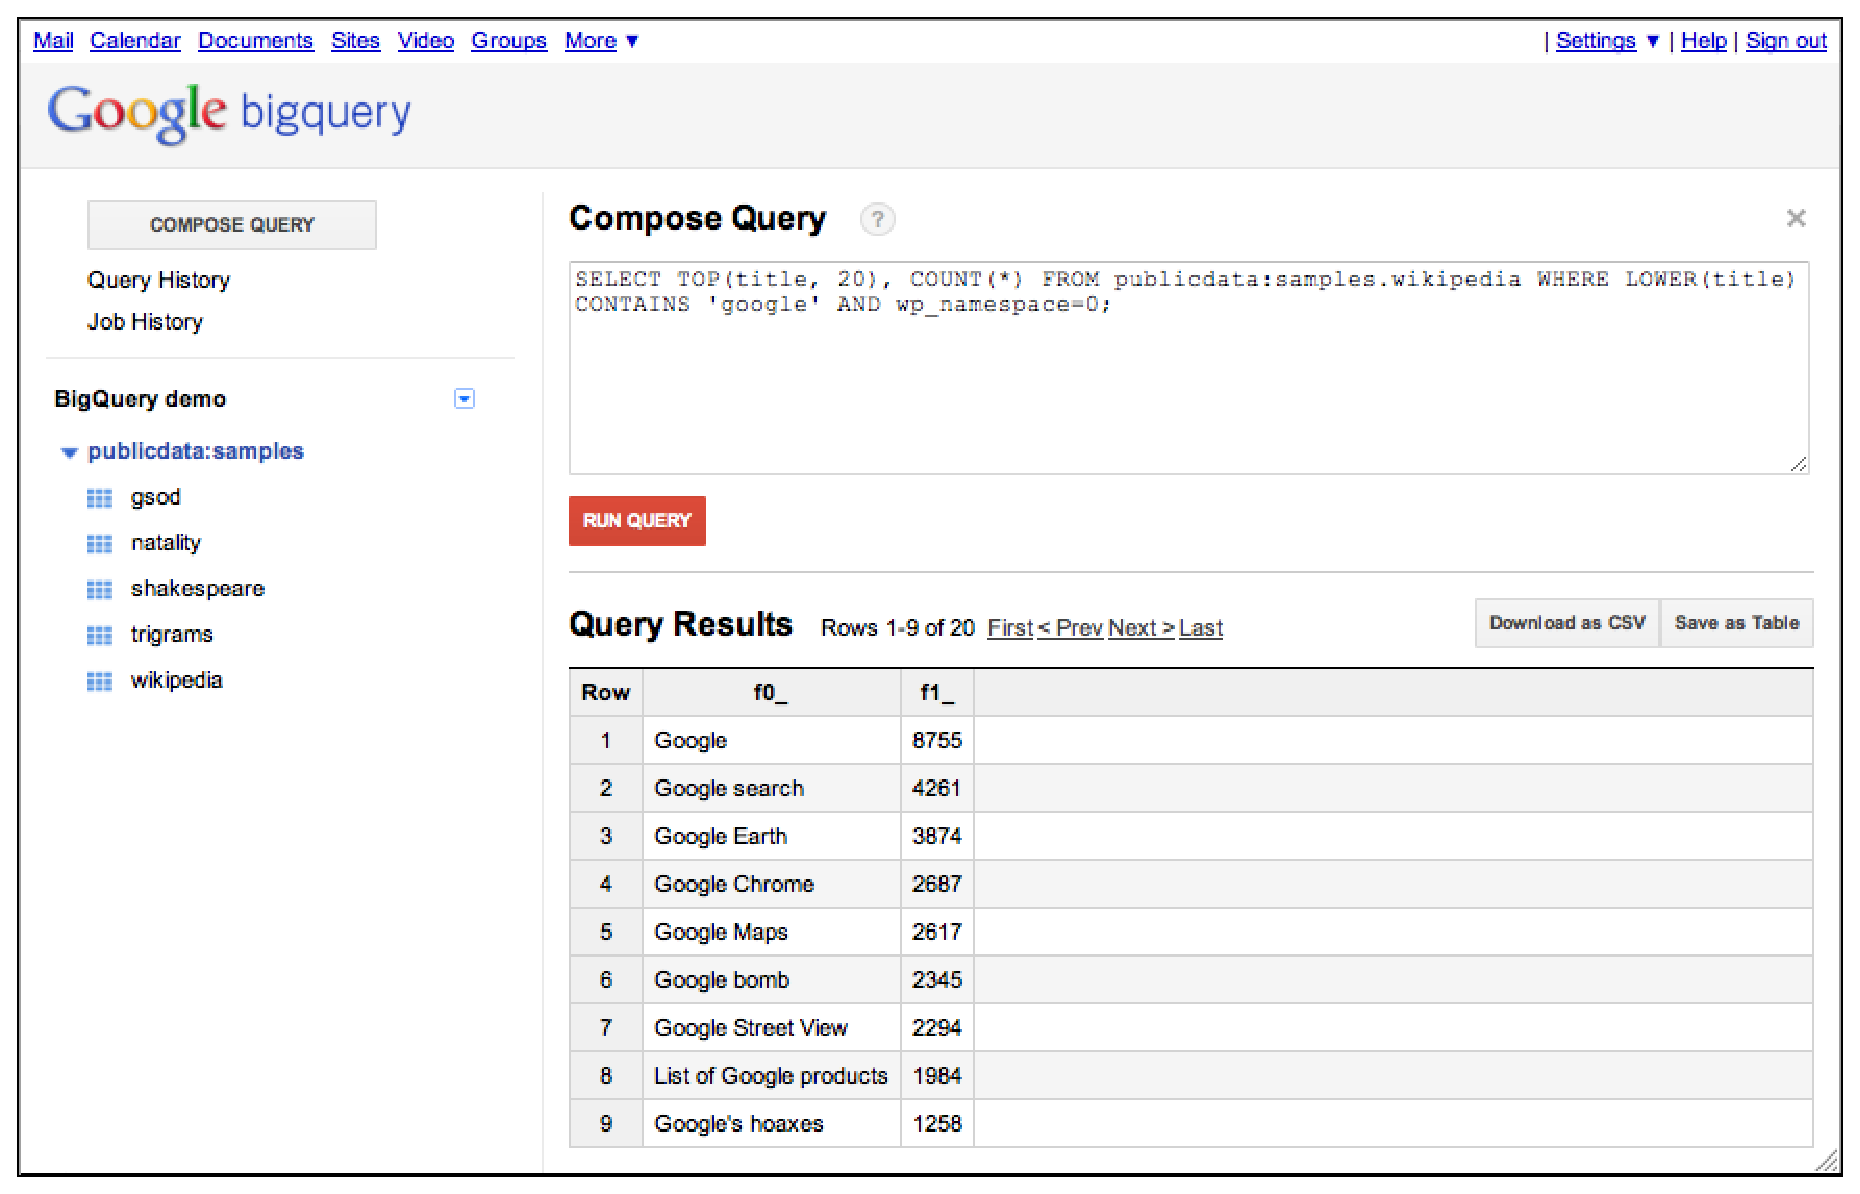
\includegraphics[width=\linewidth]{images/userinterface}}
\caption{\cite{www-userinterface-bigquery} Big Query User Interface}
\label{fig:bigqueryinterface}
\end{figure}

Figure \ref{fig:bigqueryinterface} shows the Big Query User Interface.

\subsection{Multiple permissions}
It is the capacity to manage different access permissions, read -
only, editing or owner.

\subsection{Security}
To ensure security, the solution makes use of SSL (Secure Sockets Layer)

\subsection{Multiple access methods}
We can access the service in different ways. We can use a BigQuery
Browser tool, a bq Command-line tool or a REST-based
API. \begin{itemize}
\item BigQuery Browser Tool: With this tool it is possible to easily browse,
create tables, run queries, and export data to Google Cloud Storage.
\item bq command-line Tool: This Python command - line tool permits
  to manage and query the data. \item REST API: We can access BigQuery
  making calls to the REST API using a variety of client libraries
  such as Java, PHP or Python.  \end{itemize}


\section{Experiment}

\noindent
In \cite{tajo-paper}, the performance of Tajo and Hive has been
compared by using 1TB TPC-H benchmark set. Figure
\ref{fig:experiments} shows the experimental results. For this
experiment, they have used an in-house cluster of 32 nodes, each of
which is equipped with 16GB RAM, 4TB HDD, and an Intel i5 quad core
CPU. The x-axis means the TPC-H queries and the y-axis indicates the
processing times. The results show that the time take by Tajo to
execute SQL queries is less than Apache Hive on the top of MapReduce.

\section{COST}
Many prices are practiced, existing free levels. It is charged to the
customer by the total information processed but for loading, reading or
export information there is no associated cost.  There is also budget
option for a particular project.

\section{Conclusion}
In this paper I present Google BigQuery platform, which is a
cloud-based database service that is able to process large data sets
quickly. BigQuery allows to run SQL-like queries against multiple
terabytes of data in a matter of seconds. It is suitable for ad hoc
OLAP/BI queries that require results as fast as possible. As a
cloud-powered massively parallel query database it provides extremely
high full-scan query performance and cost effectiveness compared to
traditional data warehouse solutions and appliances.

\section*{Acknowledgements}

I would like to thank my professor Gregor von Laszewski and all the
associate instructors for their constant technical support.

% Bibliography

\bibliography{references}
 
\newpage

\appendix


\end{document}
